%!TEX root = ../Report.tex

In this chapter, we present specific implementation details of the project, and cover the problems that occurred and how they were solved.

Since the system was developed incrementally, we will cover the implementation in a similar fashion, starting with the implementation of a basic skeleton function, then adding plasticity, and contention aware scheduling. Finally, we finish with the applications developed to evaluate the project.

C++ was chosen as a basis, since it's fast, and provides language constructs such as templates and overloading. Another, personal, reason is that I wished to learn something new, as I had not used C++ before. 

The parallel backend that the system is based upon is Pthreads due to its wide availability, and the level of fine control. It allows us to tune all parameters of the program and implement functions which are not possible with other solutions, e.g. detailed metric analysis. 



\section{Skeleton Foundation}
\label{section:implementation_skeleton_foundation}

The first skeleton we will implement is the map-array skeleton, as described in section \ref{section:design_skeleton_foundation}. It is reasonably straight forward to create a sequential skeleton, using c++ templates to create a templated function which takes a function amongst other things as it's arguments. This will be our skeleton. The interface of our skeleton is given in figure \ref{fig:map_array_interface}, and a usage example in figure \ref{fig:map_array_usage_example}.



\begin{figure}
	\begin{lstlisting}

	template <typename in1, typename in2, typename out>
	void map_array(deque<in1>& input1, 
				   	deque<in2>& input2, 
				   	out (*user_function) (in1, deque<in2>), 
				   	deque<out>& output, 
				   	string output_filename = "", 
				   	parameters params = parameters())

	\end{lstlisting}

	\caption{Interface of our map\_array skeleton. The first four variables are the two input arrays, the function to apply, and the output array respectively. The output\_filename variable is the filename to record the metrics output in, and params sets up the initial parameters we will use. These last two are optional.}
	\label{fig:map_array_interface}
\end{figure}



\begin{figure}
	\begin{lstlisting}

	int user_function(int in1, deque<int> in2) {
		return in1 + in2[in1];
	}

	int main() {
		// Inputs.
		deque<int> input1(ARRAY_SIZE);
		deque<int> input2(ARRAY_SIZE_2);

		/*
		 * Put data in inputs.
		 */

		// Output.
		deque<int> output(ARRAY_SIZE);

		// Start mapArray.
		map_array(input1, input2, user_function, output);

		/*
		 * Record output.
		 */
	}

	\end{lstlisting}

	\caption{A usage example of map\_array, here we apply our user\_function to each element of input1. The size of our two input arrays need not match, but the size of the input1 and output arrays must.}
	\label{fig:map_array_usage_example}
\end{figure}



\begin{minipage}{\textwidth}

Parallelizing this presents two problems, namely:

\begin{itemize}
	\item How to divide tasks amongst threads (In map array, one task is one application of the user function to an element of the input array)
	\item How many threads should be used
\end{itemize}

\end{minipage}
 
Currently in our implementation, both of these parameters must be specified beforehand and will not change at runtime. Both are aspects of the skeleton which we would like to be variable, to provide different implementations for the plasticity portion of this project. To this end, we need to implement multiple different schedules, and the ability to use a variable number of worker threads.

To implement multiple schedules, we use a bag of tasks object. A bag of tasks is a collection of independent, usually similar tasks which are to be executed. It is a model which is usually combined with some form of parallelism.

Each thread will be given the location of the same bag, and will retrieve a specified number of tasks at a time from the bag. Since each schedule is essentially consists of retrieving a different number tasks, we can use this to implement the basic schedules (Static, Dynamic chunks, Dynamic Individual). More complex schedules can easily be added in the future, as they can reuse the get tasks method, an simply adjust how many tasks each thread retrieves at one time.  

The bag also provides the main source of inter-thread communication using shared memory, and contains various semaphores for controlling the threads. This will be expanded upon in sections \ref{section:implementation_adding_plasticity} and \ref{section:implementation_contention_aware_scheduling}.

Because we use this bag of tasks object, it gives us the basis for further extensions, such as using multiple bags, adding task stealing, or adding tasks to the bag during computation.

Providing a variable amount of worker threads is simple now that we have the bag of tasks, all we need to do is to adjust our initial calculations when calculating how many tasks each thread should receive according to the schedule. These worker threads will be spawned by the original thread, the ``main'' thread. It will block until all computation is complete, it will then join with each of the worker threads.

(*** I think that the organization of these sections, particularly discussing the bag of tasks, can be organized better ***)



\section{Adding Plasticity}
\label{section:implementation_adding_plasticity}

We already have a sort of compile time plasticity in our system, in that we can choose some parameters of the skeleton before compilation. We can choose the number of worker threads and the schedule used. The other main aspect we would like to control is what CPU core each thread executes on. This is called processor affinity or thread pinning. This was added to the skeleton by adding control variables to the bag of tasks, which control the CPU affinity of each thread. Each thread then simply sets it's affinity to the intended CPU.

To add runtime plasticity, we need to be able to change the implementation of the skeleton on the fly. The most straightforward method of achieving this is to stop all computation, terminate worker threads, update the parameters, and resume computation. Previously, (as described at the end of section \ref{section:implementation_skeleton_foundation},) the main thread would block until the computation is complete, and would then join with each of the worker threads. We now change this so that, instead of blocking, it monitors the computation and can instruct the threads to terminate at any point (using the afore mentioned bag of tasks described in section \ref{section:implementation_skeleton_foundation} for communication). This allows it to prematurely terminate the computation, and then restart it with the new desired parameters. When this is done and what the new parameters should be is another matter. A future system would calculate these things dependent upon the current state of the system, but for our preliminary investigation, we manually produce them in a synthetic environment, and communicate them to the main thread using the controller application, as described in section \ref{section:implementation_contention_aware_scheduling}.

(*** Above paragraph may need to be split up, as it's pretty huge as is ***)



An obvious optimization of this system would be to modify the implementation without the need to terminate threads. This graceful switching of the implementation is left for future work, as this optimization is very complex, and would likely result in a marginal speedup proportional to the number of times we wish to change the implementation. We don't plan on switching implementations excessively, and any delay added could be overcome in testing by increasing the input size, and this project is only investigating if this approach to parallel programming is promising.



\section{Contention Aware Scheduling}
\label{section:implementation_contention_aware_scheduling}

As detailed in section \ref{subsection:design_contention_aware_scheduling} of the design chapter, we will use a separate controller application to co-ordinate and control all programs using our library. This simplifies the implementation significantly, as it gives us a single point of contact, and a single place to calculate an optimal configuration for each program. To achieve this, we need our separate controller application, and two main additions to our system:

\begin{itemize}
	\item Inter-process communication
	\item Separate communication/control thread for each program
\end{itemize}

We use the zeromq library to provide inter-process communication for it's speed, although it could be replaced with another method. It uses tcp sockets, and serves to simplify inter-process communication. Currently I have made simple use of zeromq for now, and may optimize it in the future.

In order to communicate with the controller while a program is using our library, we utilize our main thread, which will manage the worker threads, switch implementations when instructed, and will clean up after we have finished our computation. The main thread communicates with the controller, registering with it when we start and de-registering once complete. During computation, it listens to messages from the controller using non-blocking communication. This allows us to also check if we are finished processing. For the initial registration and de-registration, we use blocking communication, as these messages are vital to the system. This system is illustrated in figure \ref{fig:controller_flowchart}, and figure \ref{fig:communication_structure} shows the communication model.

\begin{figure}
	\centering
	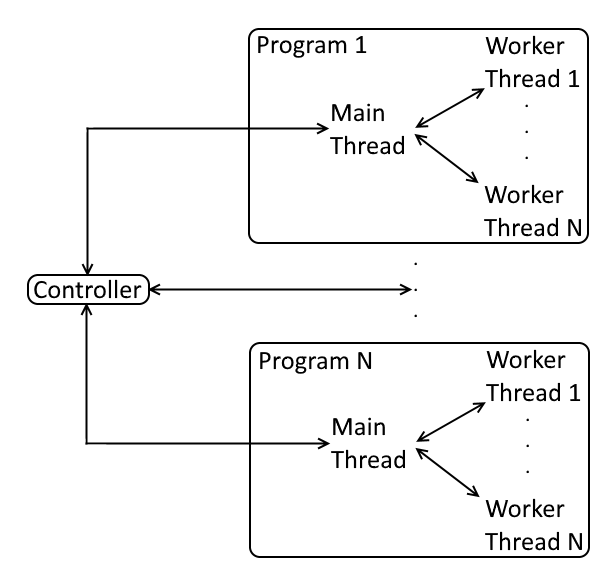
\includegraphics[width=0.8\textwidth]{graphics/communication_structure.png}
	\caption{Overall communication model of the system, with an arbitrary number of programs, with an arbitrary number of threads. Two way communication occurs between the controller and each main thread, and then between each main thread and it's worker threads.}
	\label{fig:communication_structure}
\end{figure}



\section{Evaluation}

To evaluate our library, we need programs to run and test the library under differing conditions, and we need programs to represent competing approaches to parallel programming. 

The main map-array test application is a tool which can read experiment parameters from a configuration file, and then run each experiment in sequence, recording various metrics for later analysis. This provides a convenient framework for carrying out experiments, and easily enables us to queue up a set of experiments. This is important because such experiments can take hours.

For meaningful analysis, we need to synthesize a workload. One which we can scale, so we can test different sized tasks and varying task distributions. To do this we use the Collatz function to generate a CPU intensive workload. A constant starting number is used, and the sequence is repeated multiple times, to scale the workload.

The comparison programs consist of a purely sequential implementation, and an OpenMP implementation. These were chosen because the former represents an implementation a traditional sequential programmer would use, and OpenMP because it is a popular method of parallelizing code, with a focus on performance and a simple interface. They are set up such that they can use the same synthetic workload we use for testing our library.

The final program used for evaluation is a python program which was used to create graphs from the generated data.